\vspace*{-1cm}

\nombreCapituloCabecera{RH}{Gestión y metodología del proyecto} % Título de la sección en la cabecera

\section{Gestión y metodología del proyecto} % Título del capítulo
\label{sec:gestion_y_metodologia_del_proyecto}

% ---------------------------------------------------

\subsection{Metodología de desarrollo}

El desarrollo del proyecto se ha realizado siguiendo una metodología incremental e iterativa. Este enfoque ha permitido construir el laboratorio de forma progresiva, validando cada componente antes de incorporar nuevas funcionalidades o escenarios de ataque.

En una primera fase se diseñó la arquitectura general del laboratorio y se desplegó la infraestructura básica compuesta por una máquina atacante y un servidor web vulnerable. Una vez validado el funcionamiento del entorno inicial, se incorporaron nuevos elementos con el objetivo de aumentar el realismo del escenario, incluyendo una red interna segmentada y una infraestructura Windows basada en Active Directory.

Posteriormente se implementaron las vulnerabilidades presentes en la aplicación web y se desarrollaron los distintos escenarios de explotación. Cada fase fue sometida a pruebas de validación para garantizar la estabilidad del entorno y asegurar la correcta integración de los diferentes componentes.

Este enfoque permitió identificar incidencias de forma temprana, simplificar las tareas de depuración y facilitar la evolución progresiva del laboratorio hasta alcanzar la arquitectura final propuesta.

\subsection{Planificación del proyecto}

La ejecución del proyecto se dividió en varias fases que permitieron abordar de forma estructurada las diferentes tareas necesarias para la construcción del laboratorio.

\begin{enumerate}

    \item \textbf{Análisis de requisitos y definición de objetivos.}

    En esta fase se identificaron las necesidades del proyecto, se definieron los objetivos generales y específicos del laboratorio y se establecieron los requisitos funcionales y no funcionales que debía cumplir la solución final.

    \item \textbf{Diseño de la arquitectura del laboratorio.}

    Se diseñó la estructura general del entorno vulnerable, definiendo los sistemas que formarían parte de la infraestructura, la segmentación de red, los servicios necesarios y las relaciones entre los distintos componentes. La máquina atacante queda fuera del despliegue del laboratorio y deberá ser preparada por el usuario mediante Kali Linux, Parrot OS u otra distribución equivalente.

    \item \textbf{Despliegue de la infraestructura virtual vulnerable.}

    Se procedió a la creación y configuración de las máquinas virtuales que componen el laboratorio vulnerable, incluyendo el servidor web, el controlador de dominio y la estación de trabajo corporativa.

    \item \textbf{Desarrollo de la aplicación web vulnerable.}

    Se implementó una aplicación web orientada a simular un portal corporativo realista, incorporando funcionalidades habituales de gestión de usuarios, clientes, empleados y tickets.

    \item \textbf{Implementación de vulnerabilidades y escenarios de ataque.}

    Se introdujeron vulnerabilidades de forma controlada siguiendo las categorías definidas por OWASP Top 10 y se diseñaron distintos escenarios de explotación que permitieran encadenar varias fases de ataque.

    \item \textbf{Integración de Active Directory y servicios internos.}

    Se desplegó una infraestructura Windows basada en Active Directory para simular una red corporativa interna y permitir la ejecución de técnicas de enumeración, pivoting y movimiento lateral.

    \item \textbf{Automatización del despliegue.}

    Se desarrollaron scripts y procedimientos automatizados destinados a simplificar la instalación, configuración y puesta en marcha del laboratorio vulnerable, mejorando su reproducibilidad.

    \item \textbf{Validación y documentación del entorno.}

    Finalmente, se verificó el correcto funcionamiento de todos los componentes mediante diferentes pruebas de explotación desde una máquina atacante externa y se elaboró la documentación técnica necesaria para facilitar su despliegue y utilización.

\end{enumerate}

La planificación se realizó de forma flexible, permitiendo adaptar el alcance de determinadas tareas a medida que evolucionaba el laboratorio y se identificaban nuevas oportunidades de mejora.

\subsection{Recursos utilizados}

Para el desarrollo del proyecto se han empleado diferentes recursos hardware y software destinados al despliegue de la infraestructura virtual, el desarrollo de la aplicación vulnerable.

\subsubsection{Hardware}

El laboratorio está diseñado para ejecutarse sobre un equipo anfitrión capaz de virtualizar varias máquinas de forma simultánea. Al tratarse de un entorno compuesto por varios sistemas independientes, el recurso más relevante es la memoria RAM disponible, seguida del número de núcleos de CPU y del espacio de almacenamiento reservado para los discos virtuales.

La infraestructura vulnerable desplegada está compuesta por tres máquinas virtuales principales: un servidor Ubuntu Server utilizado como servidor web vulnerable, un controlador de dominio Windows Server 2012 denominado \texttt{DC01} y una estación de trabajo Windows 7 denominada \texttt{DEV01}. Estas tres máquinas constituyen el laboratorio.

La máquina atacante no forma parte de la infraestructura vulnerable como tal, ya que puede plantearse de dos formas distintas. En primer lugar, si el equipo anfitrión utiliza un sistema operativo orientado a seguridad ofensiva, como Kali Linux o Parrot OS, el propio host puede actuar como máquina atacante. En segundo lugar, si el equipo anfitrión utiliza un sistema operativo de propósito general, como Windows, Linux o macOS, será necesario preparar una máquina virtual atacante adicional con Kali Linux, Parrot OS u otra distribución equivalente.

Los recursos mínimos recomendados para las máquinas virtuales del laboratorio son los siguientes:

\vspace{0.5cm}
\newcolumntype{C}[1]{>{\centering\arraybackslash}m{#1}}
\renewcommand{\arraystretch}{1.5}

\begin{table}[h]
    \centering
    \captionazul{Recursos mínimos recomendados para las máquinas virtuales del laboratorio}

    \setlength{\arrayrulewidth}{0.05mm}

    \begin{tabular}{|C{6.5cm}|C{2cm}|C{2cm}|C{2cm}|}
        \hline
        \rowcolor{blue!10}
        \textbf{Máquina Virtual} & \textbf{CPU} & \textbf{RAM} & \textbf{Disco} \\
        \hline
        Servidor web Ubuntu Server 22.04 & 2 cores & 3 GB & 40 GB \\
        \hline
        DC01 Windows Server 2012 & 2 cores & 4 GB & 60 GB \\
        \hline
        DEV01 Windows 7 & 2 cores & 3 GB & 40 GB \\
        \hline
        \rowcolor{red!8}
        Máquina atacante externa (opcional) & 4 cores & 3 GB & 40 GB \\
        \hline
    \end{tabular}
    \renewcommand{\arraystretch}{1}
    \label{tab:recursos_minimos_vm}
\end{table}
\vspace{0.5cm}

A partir de estos valores, el equipo anfitrión debería disponer, como mínimo, de 8 núcleos de CPU, 16 GB de memoria RAM y al menos 200 GB de espacio libre en disco para ejecutar el laboratorio con cierta fluidez. No obstante, se recomienda contar con 32 GB de RAM cuando se desee trabajar simultáneamente con todas las máquinas encendidas y realizar pruebas de explotación de forma cómoda.

En caso de que el usuario no disponga previamente de una máquina atacante, será necesario preparar una máquina adicional con una distribución orientada a seguridad ofensiva. Para este sistema se recomienda asignar 4 núcleos de CPU, 3 GB de RAM y 40 GB de disco, aunque estos recursos pueden variar en función de las herramientas instaladas y del uso previsto.

Por tanto, para un despliegue completo de la infraestructura vulnerable se recomienda que el equipo anfitrión disponga de las siguientes características:

\begin{itemize}
    \item Procesador de 8 núcleos o superior con soporte de virtualización por hardware.
    \item 16 GB de memoria RAM recomendados.
    \item 150 GB de espacio libre en disco como mínimo.
    \item Capacidad para ejecutar VMware Workstation u otra plataforma de virtualización.
\end{itemize}

\begin{figure}[H]
    \centering

    \begin{minipage}{0.48\textwidth}
        \centering
        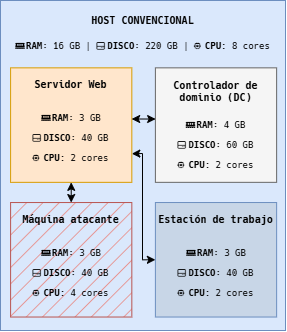
\includegraphics[width=\textwidth]{Imagenes/implementacion-VM-en-el-host.png}
        \subcaptionazul{Equipo anfitrión convencional con máquina atacante externa.}
    \end{minipage}
    \hfill
    \begin{minipage}{0.48\textwidth}
        \centering
        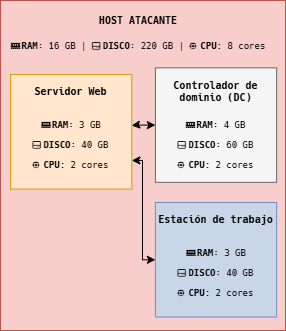
\includegraphics[width=\textwidth]{Imagenes/implementacion-VM-en-el-host-atacante.png}
        \subcaptionazul{Equipo anfitrión actuando como máquina atacante.}
    \end{minipage}

    \captionazul{Escenarios de despliegue del laboratorio: con máquina atacante externa y utilizando el propio equipo anfitrión como atacante.}
    \label{fig:escenarios_despliegue}
\end{figure}

En el caso del despliegue realizado durante el desarrollo del proyecto, el tamaño real ocupado por las máquinas virtuales fue el siguiente:

\begin{figure}[H]
    \centering
    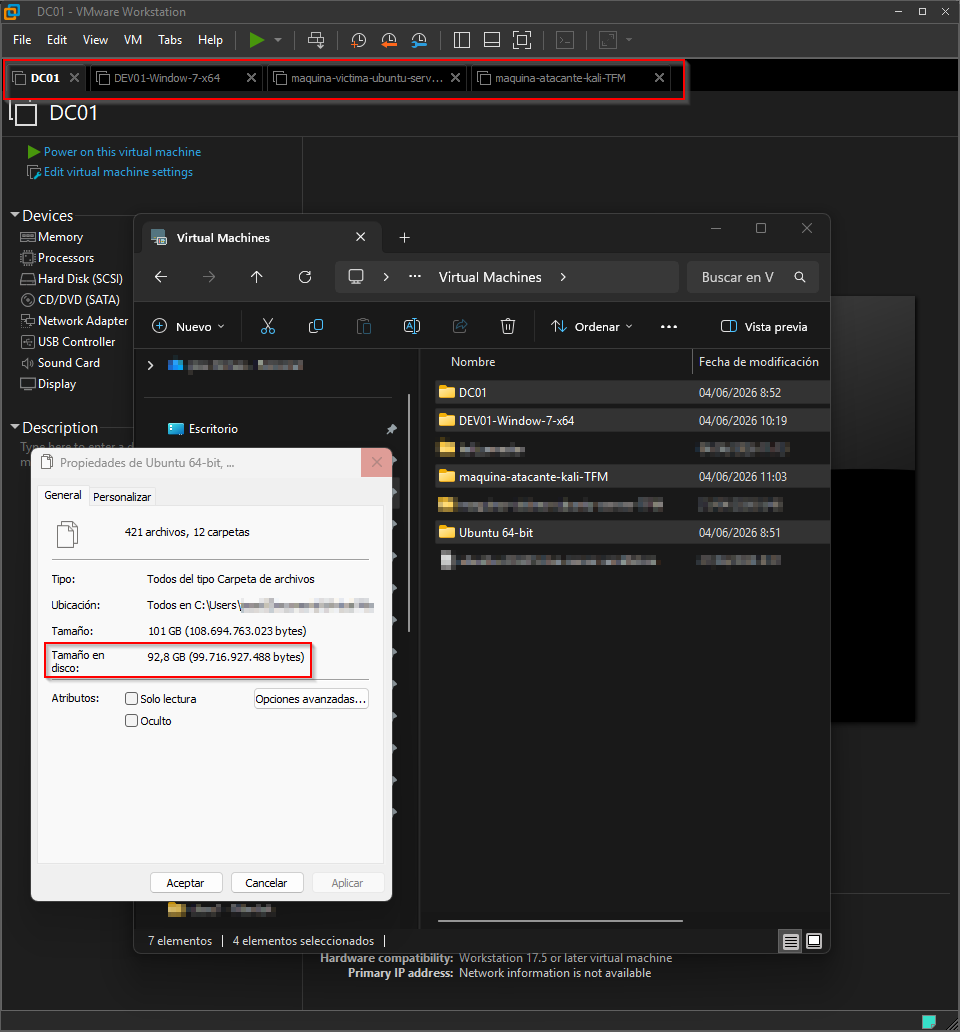
\includegraphics[width=1\textwidth]{Imagenes/tamaño-lab-en-disco-real.png}

    \vspace{0.2cm}
    \captionazul{Tamaño aproximado del laboratorio desplegado en el equipo anfitrión, incluyendo máquina atacante.}
    \label{fig:tamanio_lab_disco_real}
\end{figure}


Aunque la capacidad máxima asignada a las máquinas virtuales de la infraestructura vulnerable asciende a 140 GB, VMware utiliza discos virtuales de crecimiento dinámico, por lo que el espacio ocupado en disco depende del uso real de cada máquina.

Durante las pruebas realizadas, el laboratorio completo desplegado ocupó aproximadamente 93 GB de almacenamiento en el equipo anfitrión. Por este motivo, se recomienda disponer de al menos 150 GB de espacio libre para desplegar la infraestructura vulnerable con margen suficiente para actualizaciones, instantáneas y crecimiento de los datos.

En caso de utilizar una máquina atacante externa virtualizada, la capacidad máxima asignada al conjunto completo ascendería a aproximadamente 180 GB. Para este escenario, se recomienda disponer de alrededor de 200 GB de espacio libre en el equipo anfitrión.

\subsubsection{Software}

Para el desarrollo del proyecto se utilizaron diferentes sistemas operativos, servicios y herramientas destinados al despliegue del laboratorio, la ejecución de los componentes vulnerables y la gestión de la infraestructura virtual.

En primer lugar, se empleó \textit{VMware Workstation Pro} como plataforma de virtualización, permitiendo crear y gestionar las distintas máquinas virtuales que forman parte del laboratorio. Esta plataforma facilita la configuración de redes virtuales, la asignación de recursos hardware y el uso de instantáneas para restaurar el entorno durante las pruebas.

En relación con el servidor web vulnerable, se utilizó \textit{Ubuntu Server 22.04} como sistema operativo base. Sobre este sistema se desplegaron los servicios necesarios para alojar la aplicación web, incluyendo \textit{Apache HTTP Server}, \textit{PHP} y \textit{MySQL}. Además, se emplearon \textit{Docker} y \textit{Docker Compose} para facilitar el despliegue de los contenedores asociados al laboratorio y mejorar la reproducibilidad del entorno.

La infraestructura de directorio activo se implementó mediante \textit{Windows Server 2012}, configurado como controlador de dominio principal del laboratorio. Este sistema proporciona los servicios de \textit{Active Directory Domain Services}, DNS, SMB y WinRM, necesarios para simular un entorno corporativo Windows. Como estación de trabajo integrada en el dominio se utilizó \textit{Windows 7}, representando un equipo interno accesible desde la red corporativa.

Por último, para la gestión del código fuente y la documentación se utilizaron \textit{Git} y \textit{GitHub}, permitiendo mantener un control de versiones del proyecto, organizar los scripts de despliegue y documentar la evolución del laboratorio.


% \subsection{Coste del proyecto (opcional)}

% El desarrollo del proyecto se ha realizado utilizando principalmente software de libre distribución o licencias académicas, por lo que no ha supuesto costes económicos directos significativos.

% La mayor inversión asociada al proyecto corresponde al tiempo dedicado al diseño, implementación, validación y documentación del laboratorio. Desde una perspectiva académica, el coste puede estimarse en función de las horas de trabajo empleadas durante el desarrollo del TFM.

% Al tratarse de un entorno virtualizado y ejecutado sobre hardware previamente disponible, no ha sido necesario realizar inversiones específicas en infraestructura adicional.
